% !TEX encoding = UTF-8 Unicode
%!TEX root = thesis.tex
% !TEX spellcheck = en-US
%%=========================================
\chapter{Ontology Comparison}

\section{Loading Multiple Ontologies} % (fold)
\label{sub:loading_multiple_ontology}
In our prototype, we design the application for displaying one matching result, in order to compare different algorithm performances, we need to load multiple results at one time. Here we upgrade the main panel for loading multiple results, which is shown in Figure~\ref{fig:updated_main_panel}. 

\begin{figure*}[!ht]
	\centering
	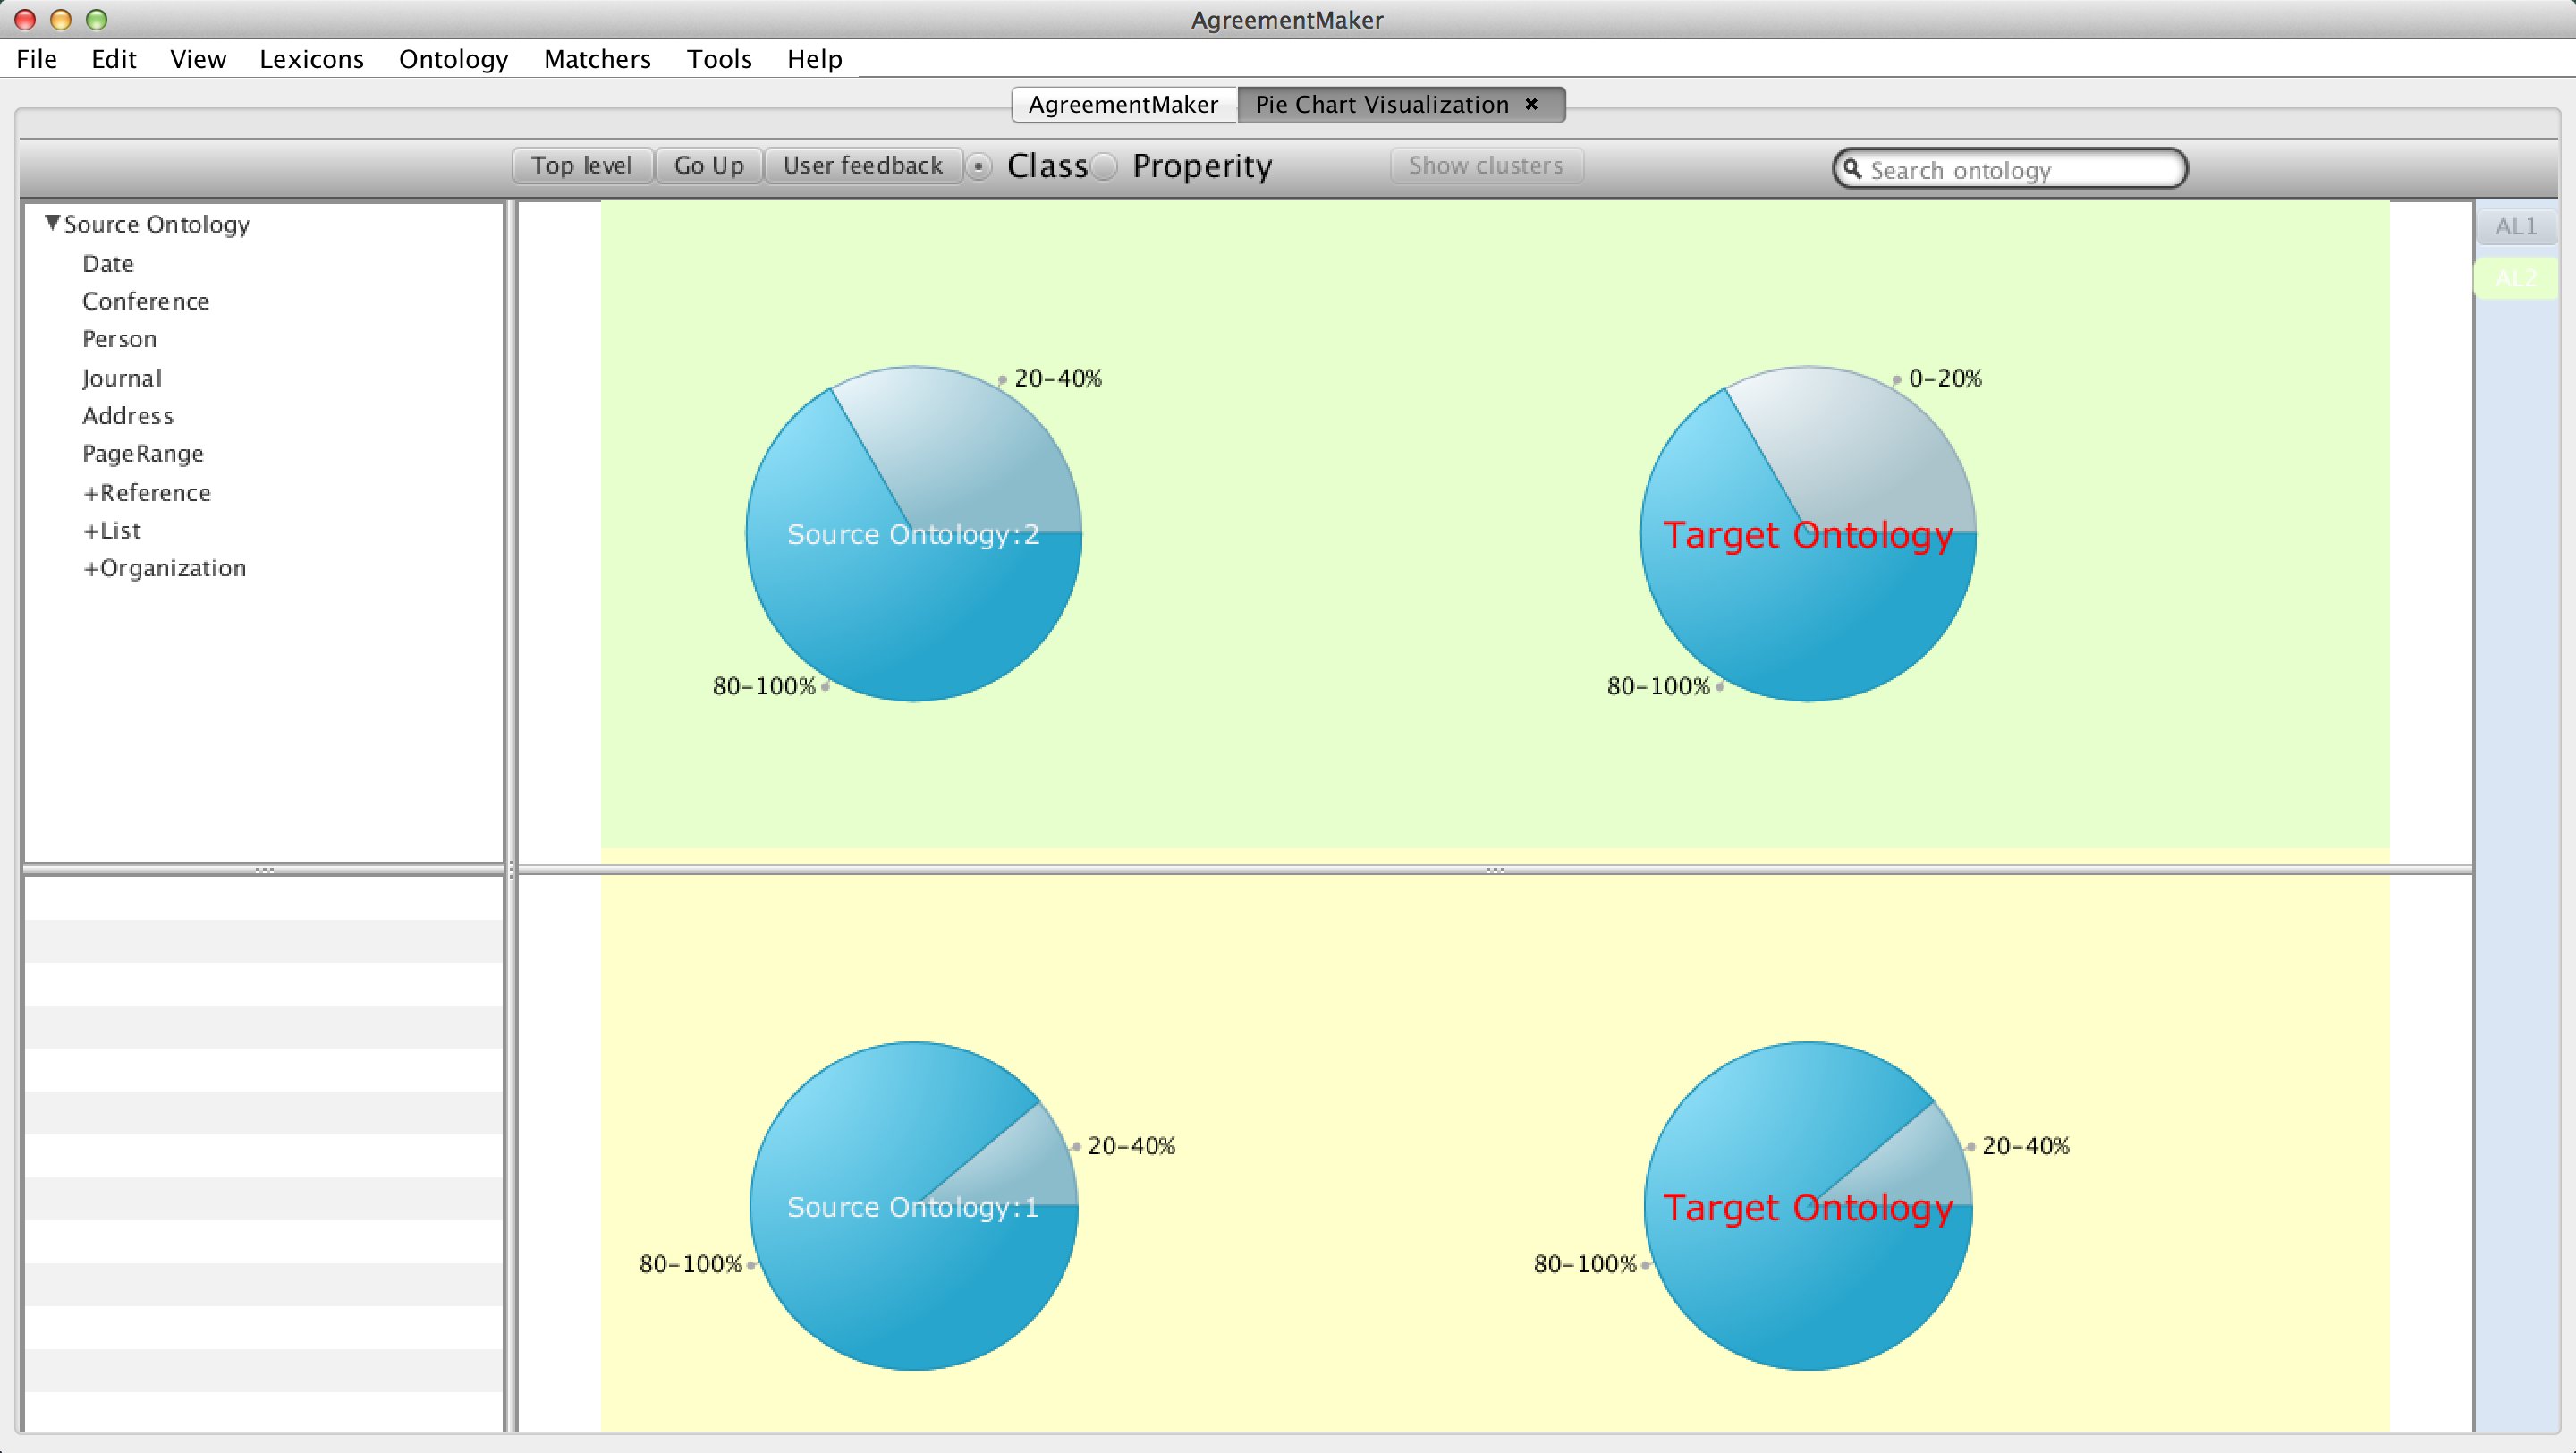
\includegraphics[width=6.5in]{pics/gui2.png}
	\caption{Updated main panel.}
	\label{fig:updated_main_panel}
\end{figure*}

We divide the main panel into two sets. The top set in green is the main set and the below set in yellow is the subset. Each set has a pair of source and target ontology. The column bar on the rightmost shows the algorithms we have loaded into the application. The main set shows the result of the second algorithm we load, which represented by the green button. The rest of the upgraded panel remains the same.

In this way, we can choose any loaded algorithm to be the main set or the subset. The difference between main set and subset is that all lists update according to the change of the main set. The reason for this design is that we have limited space on the screen panel and we need to choose the most significant information to display.

%%=========================================
\section{Comparing and Switching} % (fold)
\label{sub:comparing_and_switching}
As we mentioned above, when users click on the main set pie chart slice, all features including all pie charts and the lists will be updated. For switching the algorithm of the main set, first click on the current main set algorithm button, then click on any other algorithm button to set it as the new main set.
